\documentclass[12pt]{article}

%Bibliography   
    \usepackage{apacite}
    \bibliographystyle{apacite}
    %http://www.ctan.org/tex-archive/biblio/bibtex/contrib/apacite/apacite.pdf
 
%Essay Header
	\pagestyle{myheadings}
	\markright{\hfill \emph{Horowitz }}

%pdfLaTeX: TeX Gyre Termes
	%\usepackage{tgtermes}
	\usepackage[T1]{fontenc}

%Sectioning
    \usepackage{sectsty}
    \sectionfont{\fontsize{13}{15}\selectfont}

%Packages
    \usepackage[margin=1in]{geometry}
    \usepackage{setspace}
    \usepackage[leftmargin = 1in, rightmargin = 0in, vskip = 0in]{quoting}
    \usepackage{microtype}




\newtoggle{professormode}
%\toggletrue{professormode} %STUDENTS: DELETE or COMMENT this line



\title{MATH 390.4 Spring 2020 Homework \#1}

\author{Tziporah Horowitz} %STUDENTS: write your name here

\iftoggle{professormode}{
\date{Due 11:59PM Tuesday, February 11, 2020 under the door of KY604\\ \vspace{0.5cm} \small (this document last updated \currenttime~on \today)}
}

\renewcommand{\abstractname}{Instructions and Philosophy}

\begin{document}
\maketitle

\iftoggle{professormode}{
\begin{abstract}
The path to success in this class is to do many problems. Unlike other courses, exclusively doing reading(s) will not help. Coming to lecture is akin to watching workout videos; thinking about and solving problems on your own is the actual ``working out.''  Feel free to \qu{work out} with others; \textbf{I want you to work on this in groups.}

Reading is still \textit{required}. For this homework set, read the first chapter of \qu{Learning from Data} and the introduction and Chapter 1 of Silver's book. Of course, you should be googling and reading about all the concepts introduced in class online. This is your responsibility to supplement in-class with your own readings.

The problems below are color coded: \ingreen{green} problems are considered \textit{easy} and marked \qu{[easy]}; \inorange{yellow} problems are considered \textit{intermediate} and marked \qu{[harder]}, \inred{red} problems are considered \textit{difficult} and marked \qu{[difficult]} and \inpurple{purple} problems are extra credit. The \textit{easy} problems are intended to be ``giveaways'' if you went to class. Do as much as you can of the others; I expect you to at least attempt the \textit{difficult} problems. 

This homework is worth 100 points but the point distribution will not be determined until after the due date. See syllabus for the policy on late homework.

Up to 7 points are given as a bonus if the homework is typed using \LaTeX. Links to instaling \LaTeX~and program for compiling \LaTeX~is found on the syllabus. You are encouraged to use \url{overleaf.com}. If you are handing in homework this way, read the comments in the code; there are two lines to comment out and you should replace my name with yours and write your section. The easiest way to use overleaf is to copy the raw text from hwxx.tex and preamble.tex into two new overleaf tex files with the same name. If you are asked to make drawings, you can take a picture of your handwritten drawing and insert them as figures or leave space using the \qu{$\backslash$vspace} command and draw them in after printing or attach them stapled.

The document is available with spaces for you to write your answers. If not using \LaTeX, print this document and write in your answers. I do not accept homeworks which are \textit{not} on this printout. Keep this first page printed for your records.

\end{abstract}

\thispagestyle{empty}
\vspace{1cm}
NAME: \line(1,0){380}
\clearpage
}

\section{Silver's Book, Introduction and Chapter 1}

\begin{enumerate}

\easysubproblem{What is the difference between \emph{predict} and \emph{forecast}? Are these two terms used interchangeably today?
\ans Today, people use the terms predict and forecast interchangeably. However, if traced back to their roots, the two words are used to describe different ways of foreseeing the future. According to Silver, forecasting typically involved planning under conditions of uncertainty, much like foresight, while prediction was based on fatalism and superstition. \vspace{.5 cm}
}

\easysubproblem{What is John P. Ioannidis's findings and what are its implications?
\ans In \emph{Why Most Published Research Findings are False}, John P. Ioannidis confirms that many of the positive findings in peer reviewed laboratory experiments were likely to fail when applied in the real world. This implies that there is error in data validation. 
}

\easysubproblem{What are the human being's most powerful defense (according to Silver)? Answer using the language from class.
\ans The human being's most powerful defense is his ability to create models by observing features of reality and recognizing patterns that help him interpret his surroundings. \vspace{.5 cm}
}


\easysubproblem{Information is increasing at a rapid pace, but what is not increasing?
\ans While information is increasing at a rapid pace, useful information is not. \vspace{.5 cm}
}

\hardsubproblem{Silver admits that we will always be subjectively biased when making predictions. However, he believes there is an objective truth. In class, how did we describe the objective truth? Answer using notation from class i.e. $t,f, g, h^*, \delta, \epsilon, t, z_1, \ldots, z_t, \delta, \mathbb{D}$, $\mathcal{H}, \mathcal{A}, \mathcal{X}, \mathcal{Y}, X, y, n, p$, $x_{\cdot 1}, \ldots, x_{\cdot p}, x_{1 \cdot}, \ldots, x_{n \cdot}$, etc.
\ans The objective truth describes a phenomenon with no error. In class we denoted it as:
\begin{align*}
    y = t(z_1, z_2, \ldots , z_t)
\end{align*}
}

\easysubproblem{In a nutshell, what is Karl Popper's (a famous philosopher of science) definition of \emph{science}?
\ans According to Popper, theories can be considered scientific if they are falsifiable; meaning, they can be tested in the real world by way of prediction. \vspace{.5 cm}
}

\intermediatesubproblem{Why did the ratings agencies say the probability of a CDO defaulting was 0.12\% instead of the 28\% that actually occured? Answer using concepts from class.
\ans The rating agencies failed to accurately predict the likelihood of a CDO defaulting because they used a crude model. They did not use the proper training data because they ignored the features that were hardest to model. \vspace{.5 cm}
}

\easysubproblem{What is the difference between \emph{risk} and \emph{uncertainty} according to Silver's definitions?
\ans According to Silver, both risk and uncertainty are when the outcome depends on the assumptions and approximations you choose. The distinction between the two is in asserting the probability of the outcome. Risk is something that you can put a price on while uncertainty is much harder to measure. \vspace{.5 cm}
}

\hardsubproblem{How does Silver define \emph{out of sample}? Answer using notation from class i.e. $t,f, g, h^*, \delta, \epsilon, z_1, \ldots, z_t, \delta, \mathbb{D}, \mathcal{H}, \mathcal{A}, \mathcal{X}, \mathcal{Y}, X, y, n, p, x_{\cdot 1}, \ldots, x_{\cdot p}, x_{1 \cdot}, \ldots, x_{n \cdot}$, etc. WARNING: Silver defines \emph{out of sample} completely differently than the literature, than practitioners in industry and how we will define it in class in a month or so. We will explore what he is talking about in class in the future and we will term this concept differently, using the more widely accepted terminology. So please forget the phrase \emph{out of sample} for now as we will introduce it later in class as something else. There will be other such terms in his book and I will provide this disclaimer at these appropriate times.
\ans Silver defines \emph{out of sample} as the misspecification of the training data, $\mathbb{D}$. If features, $x_k, \ldots , x_j$ are left out of the model, there will be a higher error due to ignorance, $\delta$. \vspace{.5 cm}
}

\intermediatesubproblem{Look up \emph{bias} and \emph{variance} online or in a statistics textbook. Connect these concepts to Silver's terms \emph{accuracy} and \emph{precision}. This is another example of Silver using non-standard terminology.
\ans Statistical bias occurs when the expected value of the results differs from the true underlying quantitative parameter being estimated, i.e. the prediction is inaccurate. Variance is the measure of how far a set of numbers are spread out from their average value. The higher the variance, the less precise the prediction.
}

\end{enumerate}

\pagebreak

\section{The Theory of Modeling}

\begin{enumerate}

\easysubproblem{Redraw the illustration from lecture one except do not use the Earth and a table-top globe. The quadrants are connected with arrows. Label these arrows appropriately.
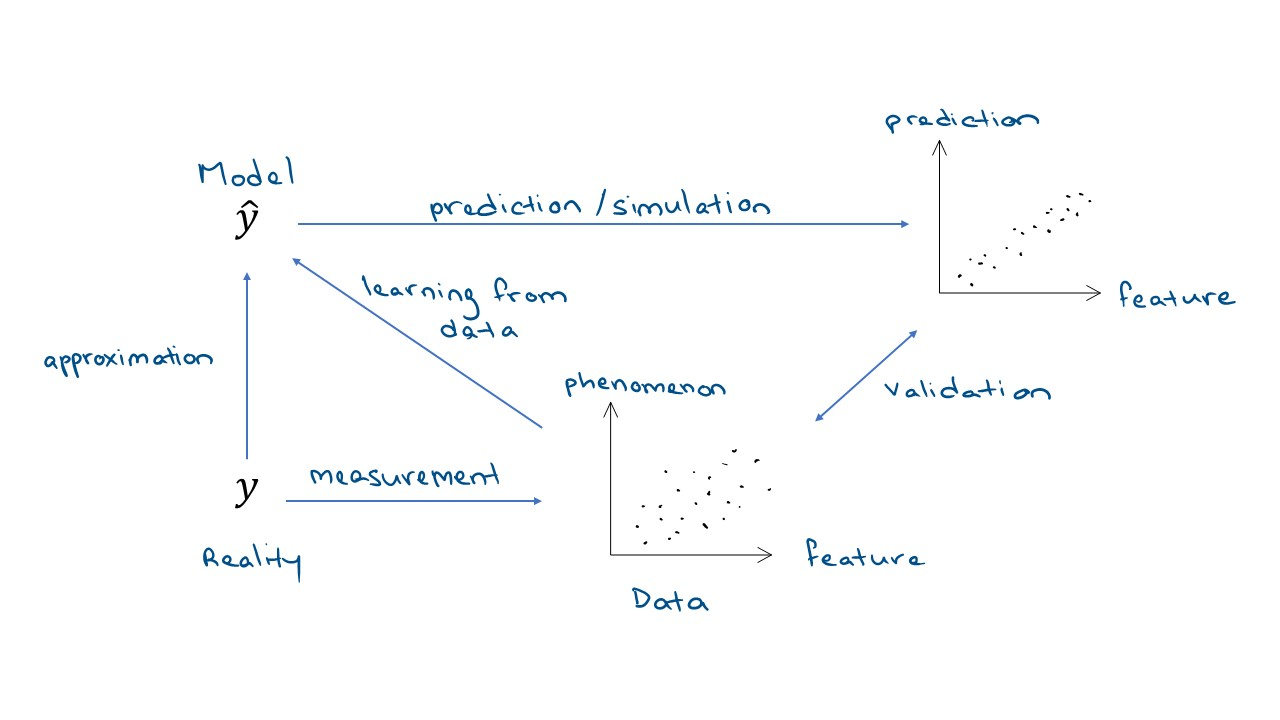
\includegraphics[width = \textwidth]{model1.jpg}
}

\easysubproblem{Pursuant to the fix in the previous question, how do we define \emph{data} for the purposes of this class?
\ans Data is the recorded result of the phenomenon based on the features measured. \vspace{.5 cm}
}


\easysubproblem{Pursuant to the fix in the previous question, how do we define \emph{predictions} for the purposes of this class?
\ans Predictions are what will happen in the real world, given the conditions of the data. \vspace{.5 cm}
}

\easysubproblem{Why are \qu{all models wrong}? We are quoting the famous statisticians George Box and Norman Draper here.
\ans All models are wrong because they are approximations of reality. The closer the approximation, the more useful the model. \vspace{.5 cm}
}

\intermediatesubproblem{Why are \qu{[some models] useful}? We are quoting the famous statisticians George Box and Norman Draper here.
\ans Some models are useful because they can explain and predict phenomena. \vspace{.5 cm}
}

\easysubproblem{What is the difference between a "good model" and a "bad model"?
\ans A good model uses metrics: it can successfully capture the phenomenon, is easily readable and unambiguous, has a good resolution, and is monotonic. A bad model is missing some or all of the metrics, making it hard to explain or predict the phenomenon. 
}

\end{enumerate}

\section{The Framework of Modeling: \qu{An Apple a Day Keeps the Doctor Away}}

\begin{enumerate}


\easysubproblem{Is this a mathematical model? Yes / no and why.
\ans This is not a mathematical model. Mathematical models are ideas and abstractions that are formulated with measurements, not physical entities. \vspace{.5 cm}
}

\easysubproblem{What is(are) the input(s) in this model?
\ans The input is eating an apple a day. \vspace{.5 cm}}

\easysubproblem{What is(are) the output(s) in this model?
\ans The output is remaining healthy. \vspace{.5 cm}
}

\intermediatesubproblem{How good / bad do you think this model is and why?
\ans This is not a good model because there are many other factors that health depends on. \vspace{.5 cm}
}

\easysubproblem{Devise a metric for gauging the main input. Call this $x_1$ going forward.
\ans $x_1$: ate 1 or more apples in 24 hours (0:00-23:59)  $\in \{0,1\}$ \vspace{.5 cm}
}

\easysubproblem{Devise a metric for gauging the main output. Call this $y$ going forward.
\ans $y$: number of doctor's visits per year $\in \naturals_0$ \vspace{.5 cm}
}

\easysubproblem{What is $\mathcal{Y}$ mathematically?
\ans $\naturals_0$ \vspace{.5 cm}
}

\easysubproblem{Briefly describe $z_1, \ldots, z_t$ in English where $y = t(z_1, \ldots, z_t)$ in this \emph{phenomenon} (not \emph{model}).
\ans $z_1, \ldots, z_t$ are the true causal inputs of phenomenon $y$. \vspace{.5 cm}
}

\easysubproblem{From this point on, you only observe $x_1$. What is $p$ mathematically?
\ans Since there is only 1 feature, $p=1$. \vspace{.5 cm}
}


\intermediatesubproblem{What is $\mathcal{X}$ mathematically? If your information contained in $x_1$ is non-numeric, you must coerce it to be numeric at this point.
\ans $\mathcal{X} = \{0,1\}$ where ate at least 1 apple is 1 and ate no apples is 0. \vspace{.5 cm}
}

\easysubproblem{How did we term the functional relationship between $y$ and $x_1$? Is it approximate or equals?
\ans Approximate relationship:
\begin{align*}
    y = f(x_1) + \delta
\end{align*}
}


\easysubproblem{Briefly describe \emph{supervised learning}.
\ans Supervised learning is obtaining $f$ by learning from data. \vspace{.5 cm}
}

\easysubproblem{Why is \emph{supervised learning} an \emph{empirical solution} and not an \emph{analytic solution}?
\ans Supervised learning is an empirical solution because it approximates the model based on data. There is no analytical solution that can be used. \vspace{.5 cm}
}

\intermediatesubproblem{From this point on, assume we are involved in supervised learning to achieve the goal you stated in the previous question. Briefly describe what $\mathbb{D}$ would look like here.
\ans $\mathbb{D}$ is the set of $n$ historical examples of the simultaneous occurrence of $x_1$ and $y$ such that:
\begin{align*}
    \mathbb{D} = \langle \mathbf{X}, \mathbf{y} \rangle
\end{align*}
Where $\mathbf{X}$ is the matrix of inputs and $\mathbf{y}$ is the vector of outputs. \vspace{.5 cm}
}

\intermediatesubproblem{Briefly describe the role of $\mathcal{H}$ and $\mathcal{A}$ here.
\ans $\mathcal{H}$ is the set of candidate functions for $f$ such that $f : \mathbf{X} \rightarrow \mathbf{y}$ and $\mathcal{A}$ is an algorithm that takes in data $\mathbb{D}$ and set $\mathcal{H}$, and produces a model $g$ such that $g = \mathcal{A}(\mathbb{D}, \mathcal{H})$. \vspace{.5 cm}
}

\easysubproblem{If $g = \mathcal{A}(\mathbb{D}, \mathcal{H})$, what should the domain and range of $g$ be?
\ans The domain is $\mathbb{R}$ and the range is $\naturals_0$. \vspace{.5 cm}
}

\easysubproblem{Is $g \in \mathcal{H}$? Why or why not?
\ans $g \in \mathcal{H}$ because $g$ is the best candidate function that $\mathcal{A}$ can produce and $\mathcal{H}$ is the set of all candidate functions for the model. \vspace{.5 cm}
}

\easysubproblem{Given a never-before-seen value of $x_1$ which we denote $x^*$, what formula would we use to predict the corresponding value of the output? Denote this prediction $\hat{y}^*$.
\ans
\begin{align*}
    \hat{y}^* = g(\x^*)
\end{align*}
}

\intermediatesubproblem{Is it reasonable to assume $f \in \mathcal{H}$? Why or why not?
\ans No, because there is error in modeling. \vspace{.5 cm}
}

\easysubproblem{In the general modeling setup, if $f \notin \mathcal{H}$, what are the three sources of error? Copy the equation from the class notes. Denote the names of each error and provide a sentence explanation of each. Denote also $e$ and $\mathcal{E}$ using underbraces / overbraces.
\ans
\begin{align*}
    y = g(\Vec{x}) + \big(h^*(\Vec{x}) - g(\Vec{x})\big) + \big(f(\Vec{x}) - h^*(\Vec{x})\big) +  \big(t(\Vec{z}) - f(\Vec{x})\big)
\end{align*}
\begin{enumerate}
    \item \textbf{Error due to ignorance}: $\delta = t(\Vec{z}) - f(\Vec{x})$, the difference between reality and the approximation of $f$.
    \item \textbf{Misspecification Error}: $f(\Vec{x}) - h^*(\Vec{x})$, the difference between the best function and the closest possible model.
    \begin{itemize}
        \item $\mathcal{E} = \big(f(\Vec{x}) - h^*(\Vec{x})\big) +  \big(t(\Vec{z}) - f(\Vec{x})\big)$
    \end{itemize}
    \item \textbf{Estimation error}: $h^*(\Vec{x}) - g(\Vec{x})$, the difference between the closest possible model and the best model that algorithm $\mathcal{A}$ finds.
    \begin{itemize}
        \item $e = \big(h^*(\Vec{x}) - g(\Vec{x})\big) + \big(f(\Vec{x}) - h^*(\Vec{x})\big) +  \big(t(\Vec{z}) - f(\Vec{x})\big)$
    \end{itemize}
\end{enumerate} \vspace{.5 cm}
}

\easysubproblem{In the general modeling setup, for each of the three source of error, explain what you would do to reduce the source of error as best as you can.
\ans \begin{enumerate}
    \item \textbf{Error due to ignorance}: measure more $x_j$'s of the units that contain information about $\Vec{z}$.
    \item \textbf{Misspecification Error}: expand $\mathcal{H}$ to include more complicated functions.
    \item \textbf{Estimation error}: increase the sample size.
\end{enumerate}
}

\pagebreak

\intermediatesubproblem{In the general modeling setup, make up an $f$, an $h^*$ and a $g$ and plot them on a graph of $y$ vs $x$ (assume $p=1$). Indicate the sources of error on this plot (see last question). Which source of error is missing from the picture? Why?
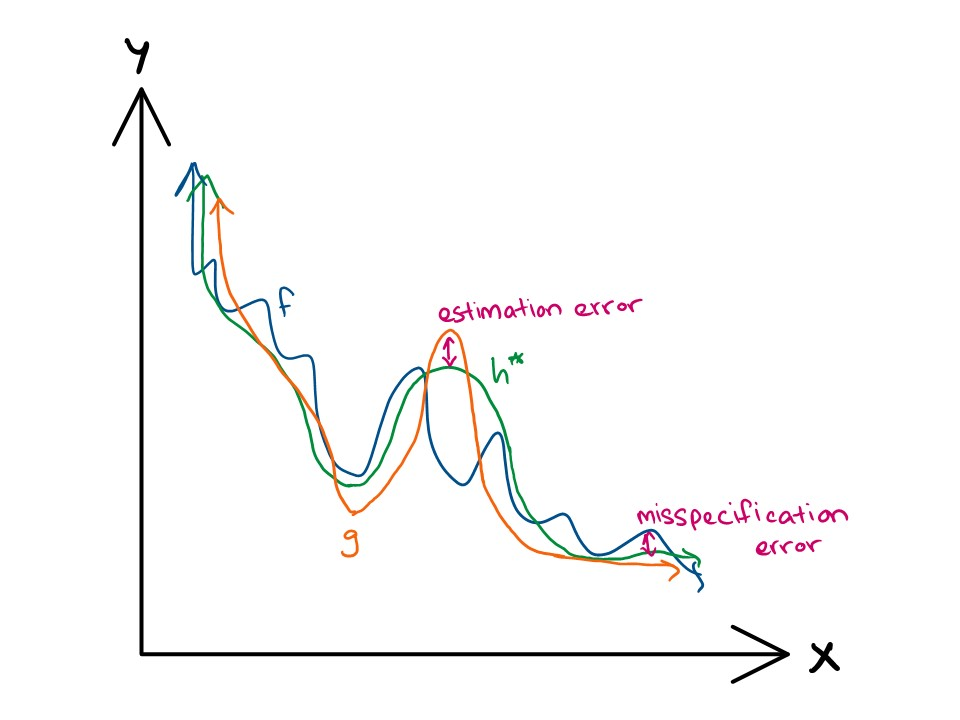
\includegraphics[width = \textwidth]{errors.jpg}
\ans The error missing from the picture is the error due to ignorance. This is because the true function, $y = t(z_1, \ldots , z_t)$ is unknown.
}



\end{enumerate}

\end{document}

